\section{Struttura middleware} \label{struttura_middleware}

Synapsis è stato realizzato utilizzando il framework Play, illustrato nella sezione \ref{play}, le cui peculiarità sono la modularità e la distribuzione, raggiunte grazie all'utilizzo del sistema ad attori ed il modello computazionale associato: Event-driven/Message-driven. 

\medskip

Un sistema asincrono basato sui messaggi può utilizzare in modo più efficiente le risorse di un sistema poiché consuma risorse, come i thread, solo quando è effettivamente necessario. I messaggi possono essere recapitati anche a macchine remote (trasparenza della posizione), man mano che i messaggi vengono messi in coda e recapitati all'attore \cite{akka-book}.

\medskip

Il sistema ad attori ha portato alla definizione di un'entità "copia" all'interno del middleware, strutturata allo stesso modo dell'entità "esterna" presente in parte su GE ed in parte su MAS.

\medskip

Questa soluzione ha semplificato concettualmente la gestione delle entità esterne da parte del middleware. Difatti, realizzando rispettivamente un attore che identifica il corpo ed un attore che rappresenta la mente è venuta meno la realizzazione di una componente logica per lo smistamento dei messaggi ricevuti dall'esterno. Ad esempio, quando un attore "mente" riceve un messaggio dall'esterno è consapevole che tale messaggio è stato generato ed inviato dall'entità "mente" e, di conseguenza, è chiaro che il destinatario è l'attore "corpo", che a sua volta invia il messaggio all'entità "corpo" esterna.

\begin{figure}[H]
\centering
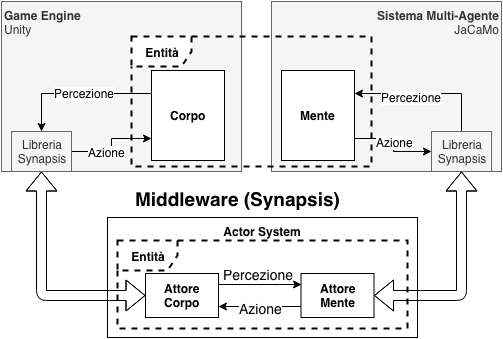
\includegraphics[width=\textwidth]{figures/Middleware_associazione_entita.png}
\caption{Associazione tra entità "esterna" ed "interna"}
\label{middleware_associazione_entita}
\end{figure}

Lo schema (figura \ref{middleware_associazione_entita}) illustra il concetto appena definito unito alla precedente architettura di sistema, dove ad ogni entità esistente nei sistemi MAS e GE viene associata una coppia di attori "mente" e "corpo" all'interno del middleware.
